\chapter{Evaluation}
\label{cap6}

Intro to evaluation, description of the three parts and why they are important/complementary (limitations!)




\section{Generality}\label{applicability}

We developed our programming framework thinking about indoor applications utilizing nano-drones.
Actually, since we work at a sufficiently high level of abstraction, because we can use an API which make the drones navigate in the environment, the model can be extended to almost every kind of drone, aerial terrestrial and aquatic.
\\
So, we can say that the Pluto programming framework is "drone independent", and this greatly extends its applicability, including also outdoor, aquatic and terrestrial environments; it is in charge of the programmer to manage the interaction between Pluto and the specific type of drone he wants to use for the particular application he's developing.

Pluto is fully exploited when there is a team of drones to manage (see \ref{fig:WIS} and \ref{fig:DD}), although it perfectly works also in the case of a single drone (see \ref{fig:OF}).
\\

Since we decided to use a Team-level approach (see \ref{teamlevel}), our model can be used for developing applications where the user can give to the system a set of actions to be performed; the dispatching of these actions is managed by the "central brain", which takes care of assigning the drones to the action and to handle all the exceptions (battery low, crashes etc.). So, the drones are only actuators that perform an action, there is no communication between them, their behavior is monitored and decided by the central brain.
\\

Since drones cannot communicate between them, Pluto cannot be used for applications where drones must perform some kind of action requiring explicit communication or data exchange between them; the logic is managed by the central brain, so communication between drones is always mediated by this component; a drone can send data to the central brain, and this could send again that data to another drone.
\\
Hereinafter we analyzed some already existing example applications, showing whether they can be managed/developed with the Pluto programming framework or not.
\\

\subsection{Object Finder, Warehouse Item-Finder, Drugs Distribution}



\subsection{Alfalfa Crop Monitoring and Pollination}\label{alfalfa}

The Alfalfa Crop Monitoring and Pollination\cite{alfalfa} is a typical example of swarm-level approach application.
Alfalfa is an important food crop for cattle and requires an external pollinator (e.g. bees) to produce seeds. In recent years, colony collapse disorder has devastated honeybee populations and jeopardized the cultivation of important crops\cite{colony}.
A swarm of drones can pollinate the alfalfa plants and also monitor them for pests and diseases, trough visual spot checks.
\\
So, the whole application provide three periodic actions: searching for pests, searching for diseases, and looking for flowers in bloom.
Each one of these actions is achieved by taking pictures of the plants.
The user may need to define time constraints within the pollination action must be completed.

The following Pluto Editor graph describes the behavior of the Alfalfa Crop Monitoring and Pollination\cite{alfalfa} application:

\begin{figure}[H]
  \centering
  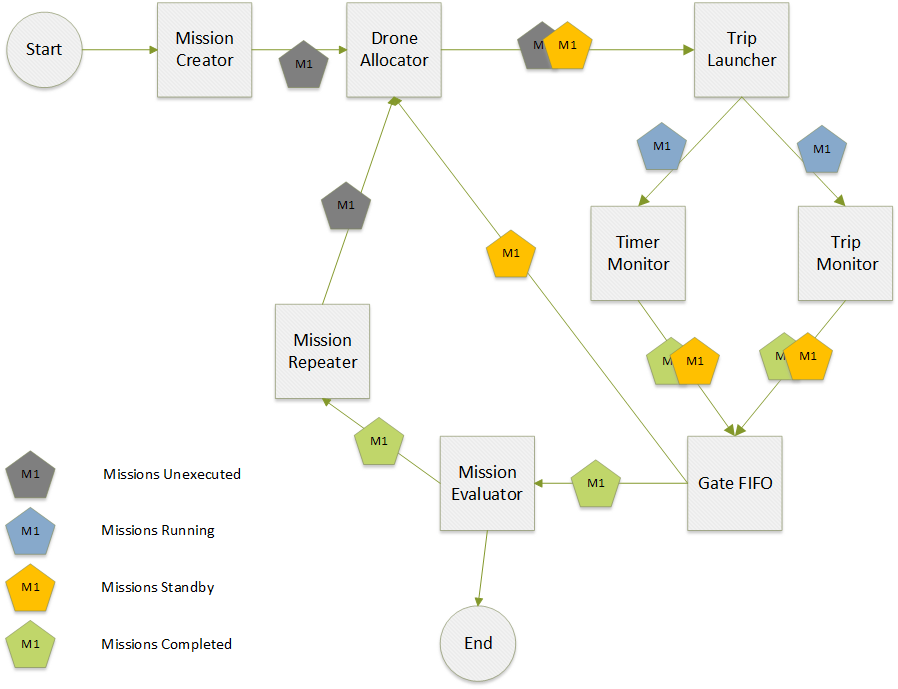
\includegraphics[width=\linewidth]{pictures/Alfalfa_Diagram.png}
  \caption{Pluto graph for the Alfalfa Crop Monitoring and Pollination application}
  \label{fig:alfalfaGraph}
\end{figure}

Thanks to the \textit{Take photo} action, already implemented in Pluto, the drones are able to perform the monitoring of leaves for pests, diseases and flowers in bloom.
\\

The flow starts with the MissionCreator block, that creates a Mission instance to propagate in the graph.
As already explained, a Mission is a list of sensing tasks to be executed sequentially.
Then the DroneAllocator block takes care of assigning the right Drone to the next Trip in the list of trips to be executed of the Mission entity.
A Trip is nothing but a movement of the Drone from a point A to a point B in the environment, at the end of which the Drone performs an Action.
Then the Mission entity arrives to the TripLauncher that simply starts the execution of the first Trip and sets the its status to RUNNING.
\\

After the TripLauncher the Mission entity is doubled. One instance goes to the TripMonitor block and the other one to the TimerMonitor.
The TripMonitor changes the status of the executing Trip depending on the outcome of the Drone's journey:
if the Drone accomplishes to complete the journey and perform the Action, then the Trip status is set to COMPLETED,
if the Drone crashes the Trip status is set to FAILED.
The time constraints, which are set by the user thanks to the \textit{timer} attribute of the Mission entity, are fulfilled thanks to the TimerMonitor block.
This block takes care of setting the Mission status to FAILED if one of its Trips is not completed within the timer.
\\

The GateFIFO block takes as input two Mission instances, one from the Trip Monitor and the other one from the Timer Monitor.
It takes care of propagating only the first instance that arrives to it.
For example, if the timer has expired then it propagates the Timer Monitor instance, otherwise the Trip Monitor one.
\\

After the GateFIFO block there is a bifurcation:
if the Mission is completed, it is sent to the MissionEvaluator, otherwise there are some trips of the mission that must be executed again, and so the Mission is sent to the DroneAllocator, which will assign new drones to these trips.
\\

The MissionEvaluator block enables the evaluation of the photos taken by the drones. If the pest and/or disease attributes are true, the system notifies the farmer of the damaged location, adding a log line in the console of the Monitor Page of the Pluto User Interface.
If the bloom attribute is true, a new Trip will be created and a new Drone, capable to perform the Pollinate action, will be sent to that location to pollinate the flowers.
\\

The Mission Repeater block takes care of continuously sending the drones to monitor these locations.
Regarding the "Pollination" task, it can be added thanks to the \textit{custom action} feature, through which the programmer can add to the model a brand new Action, making use of a specific external API.
The full explanation of the functionality of each block can be found in Section \ref{functionalBlocks}.
\\

Concerning the pictures evaluation to detect pests, diseases and flowers in bloom, the developer has to add the custom code in the Evaluator class, using again an external API. 
Each photo will have three associated parameters: the boolean attributes \textit{pest}, \textit{disease} and \textit{bloom}.
These attributes are false by default and they are set to true when the leaves are damaged, their color turns greenish-white or the flowers are in bloom, respectively. 
\\

The following is the code of the Evaluator needed for the development of the Alfalfa\cite{alfalfa} application:
"dataMap" is an hashmap that binds each Trip with the picture taken. 
The Trip is the key, which represents the journey performed by the drone, the Photo is the value, which is the picture taken by the drone once the Trip has been completed.
For each photo, if the \textit{pest} or the \textit{disease} attributes are true, the system will signal to the farmer the location where the problem exists, through the log function.
If the \textit{bloom} attribute is true, the plants at that location must be pollinated: a new Trip entity is created, its Action is set to "Pollinate" and the target location is set to the same location of the Drone that found the bloom.
Finally the Trip is added to the list of trips of the current mission.
The Mission status is set to STANDBY because there is at least a new inserted Trip to execute.
\\


\begin{lstlisting}
		String result = null;

		// Retrieve all entries of the map, it means we are iterating
        // all the completed Trips that wrote their result in the Evaluator
		for (Map.Entry<Trip, Object> entry : dataMap.entrySet()) {

			// we need to consider only the Trips related to the current
           // mission we are evaluating
			if (missionToEvaluate.getCompletedTrips().contains(entry.getKey())) {
				
				// retrieve the Photo related to the current Trip
				Photo photo = (Photo) entry.getValue();
				
				if (photo.hasPest() || photo.hasDisease())
					
					return "WARNING: Pest/disease at location: "
							+ entry.getKey().getTargetLocation();

				if (photo.hasBloom()) {

					// create a new Trip to pollinate the flowers
					Trip trip = new Trip();
					trip.setName("PollinateTrip");
                    
                    // Set the same target location
                    // of the Trip that has found the flowers
					trip.setTargetLocation(entry.getKey().getTargetLocation());
                    
                    // This action must be implemented by the developer
					trip.setAction(Action.POLLINATE);
                    
                    // the status WAITING means that this Trip
                    // is ready to be launched
					trip.setStatus(Trip.WAITING);

					// adding this Trip to the Trip list
                    // that contains all the Trips to be launched
					missionToEvaluate.getTrips().add(trip);
                    
					// The status STANDBY means that the mission
                    // has some Trips to be executed
					missionToEvaluate.setStatus(Mission.STANDBY);
				}
			}
		}

		// Result is a "success" because all the Photos of this 
        // mission have been evaluated
		result = "Success";
        
		return result;
\end{lstlisting}

To concretely choose the specific locations to monitor, the user is provided with a map over which he can drag and drop the action \textit{Take photo}.
As already explained, a Mission object contains a list of trips to be executed.
Inside the Mission entity, these trips are performed sequentially, in general each one by a different Drone, as already explained in Section \ref{programmingModel}.
So, if the user wants to send more than one drone simultaneously on the same location, he has to create more than one Mission.
Indeed missions are executed in parallel, so if the user wants to simultaneously send 3 drones on the same location, he simply has to create three missions.
Then,  since each Mission has its own Trips Page, he has to choose the same locations on the maps of the three Trip pages.
\\

To further clarify the development of the Alfalfa\cite{alfalfa} application with Pluto, we now show a real execution of the Alfalfa application in a concrete scenario:
imagine we want to simultaneously send three drones to monitor the plants distributed in a circular area.
So, we create three Mission entities, and, for each of them, we drag and drop the action \textit{Take photo} on the map of its Trip page, in order to create the trips composing the circular area, as shown in figure \ref{fig:alfalfaArea}.
The figure \ref{fig:alfalfaArea} represents the trips of one of the three Missions.
Each one of the three missions has its own map where the user distribute the trips to perform.
Then, when the missions start, the drones will take photos over these spots and, in case of bloom, new Trips will be created to Pollinate the area.

\begin{figure}[H]
  \centering
  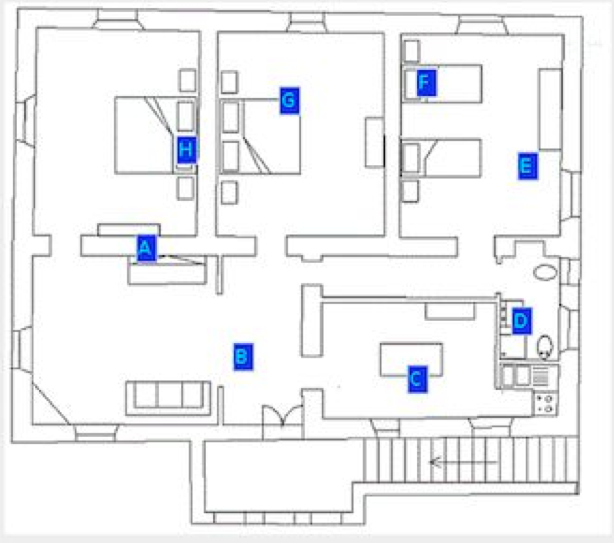
\includegraphics[width=\linewidth]{pictures/alfalfaArea.png}
  \caption{The circular area to monitor}
  \label{fig:alfalfaArea}
\end{figure}


To describe in a detailed way the execution flow, we now show the sequence diagrams of the Pluto Main Application behavior:
\\

\begin{figure}[H]
  \centering
  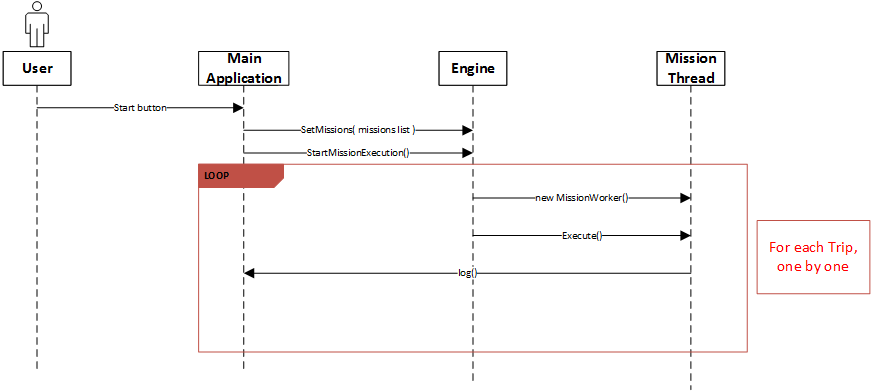
\includegraphics[width=\linewidth]{pictures/Alfalfa_Sequence_MissionStart.png}
  \caption{Sequence diagram of a starting mission}
  \label{fig:alfalfaSequence1}
\end{figure}

In figure \ref{fig:alfalfaSequence1} we show the first calls after the user clicks on the Start button in the Monitor Page.
The Main Application receives the start command from the user, then activates the Engine entity. Now, a new Thread is created and started for each missions. The status of the Missions are sent to the Pluto Main Application and showed to the final user, through the \textit{log()} function.
\\

\begin{figure}[H]
  \centering
  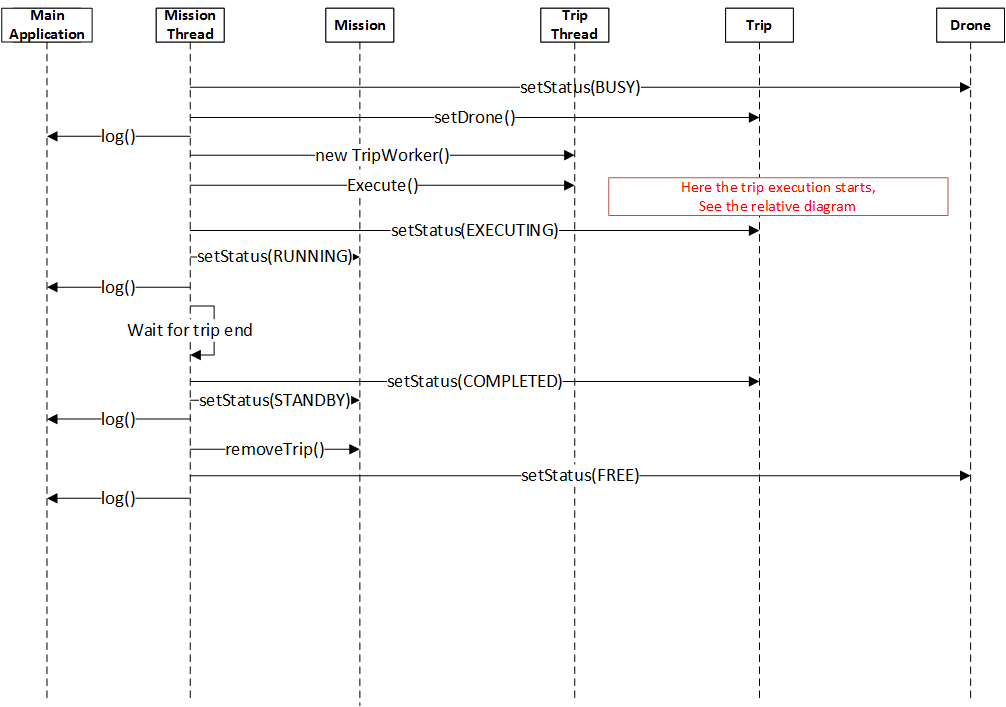
\includegraphics[width=\linewidth]{pictures/Alfalfa_Sequence_MissionExecution.png}
  \caption{Sequence diagram of the mission execution flow}
  \label{fig:alfalfaSequence2}
\end{figure}

In figure \ref{fig:alfalfaSequence2} the Mission Execution is shown.
The \textit{Mission Thread} entity manages the Mission flow through all the blocks and the execution of the logic inside them.
For example, the first two method calls belong to the Drone Allocator. 
For each Trip a new \textit{Trip Thread} instance is created, that will manage the parallel execution of the trips.
After that, the mission thread waits for the completion of the started Trip, and then the Mission Status is set to STANDBY, since there are other trips to be executed.
Finally, the completed Trip is removed from the list of trips to be executed and the Drone status is set to FREE.
Otherwise, if the launched Trips was the last one, the Mission status would have been set to COMPLETED.
\\

\begin{figure}[H]
  \centering
  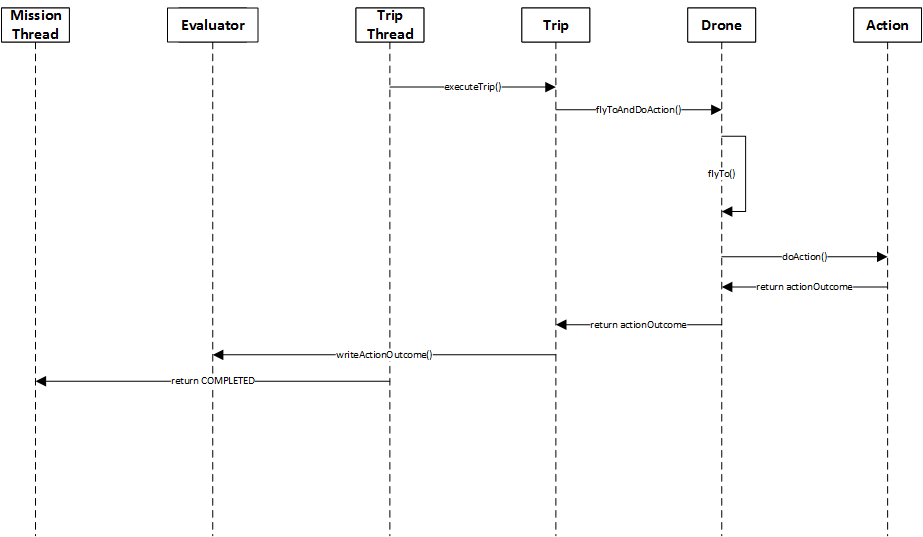
\includegraphics[width=\linewidth]{pictures/Alfalfa_Sequence_TripExecution.png}
  \caption{Sequence diagram of the trip execution flow}
  \label{fig:alfalfaSequence3}
\end{figure}

In figure \ref{fig:alfalfaSequence3} the Trip execution is shown.
The Drone assigned to the Trip is sent to the established location to take the pictures.
After that, the resulting photo is written into the Evaluator entity, where the specific algorithm of the application will perform the evaluation, once the mission will be completed.
\\

\begin{figure}[H]
  \centering
  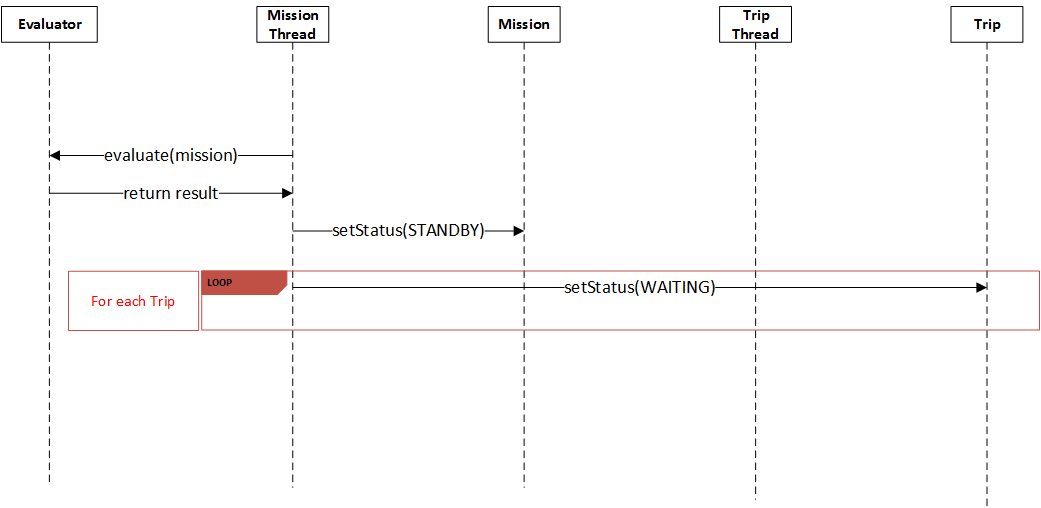
\includegraphics[width=\linewidth]{pictures/Alfalfa_Sequence_MissionEnd.png}
  \caption{Sequence diagram of the mission ending flow}
  \label{fig:alfalfaSequence4}
\end{figure}

In figure \ref{fig:alfalfaSequence4} the final steps of the Mission execution are shown.
The \textit{Evaluator} checks the pictures taken by the Drones, looking for pest, diseases or blooms.
The Trips are re-inserted in the execution list, their status is set to WAITING,and the Mission status is set to STANDBY because of the MissionRepeater block.
The MissionRepeater takes care of executing again a Mission, and to do so the status of the Mission must be STANDBY.
\\

\subsection{Aerial mapping of archaeological sites}\label{aerialMapping}

This application allows archaeologists to survey ancient sites without involving their direct presence on it.
Many ortophotos of the site are taken, so that the archaeologists can see the geometric layout of the site, without physically walking near it, which could cause irreparable damages.
An orthophoto is an aerial photo that is geometrically-corrected so that distances between pixels are proportional to true distances, such that the photo can be used as a map.
Drones are sent to take a series of ortophotos that then will be stitched together to derive a single ortophoto; if the individual pictures do not have sufficient overlap, the resulting orthophoto will show excessive aberrations, and, in that case, the drone is sent out again to take more pictures.
If the obtained ortophoto is not adequate, the archaeologists should be able to send more drones on that particular area.
The drones must perform their actions in a limited amount of time, since if too much time pass between two ortophotos, the scene may change.

Regarding the Pluto graph needed for this application, it is very similar to the Alfalfa\cite{alfalfa} application one, shown in figure \ref{fig:alfalfaGraph}.
The only difference is the absence of the MissionRepeater block, since this application does not need the drones to repeat their tasks continuously.
So, in the graph of the "Aerial mapping of archaeological sites" application the MissionEvaluator block is directly connected to the DroneAllocator.
\\

The flow of the Mission entity on the graph is the same of the Alfalfa\cite{alfalfa} application, and is fully described in section \ref{alfalfa}.
In this case the MissionEvaluator block analyzes the drones data at the end of the missions, allowing the Main Application to decide if the photos are good enough or if more drones must be sent out to take new pictures in these locations.
\\

It is important to underline that, using the Pluto framework, it is not possible to obtain the very same behavior of the original application.
Indeed, two consecutive photos must be taken within a time constraint.
This cannot be fulfilled with Pluto, since the TimerMonitor block deals with a time interval that starts when the drone leaves the base station, ensuring that it will take the picture before the time interval expires.
So, there is no way to state a time constraint between two consecutive photos.
\\


Concerning the code of the Evaluator block needed for the development of the Aerial Mapping\cite{putti} application, as for the previous application, we can find each photo taken during the missions in the "dataMap" parameter, that is an hashmap that create a relation between a Trip and the photo taken through its Action.
First of all, the ortophotos are stitched together to obtain the final ortophoto, trough the \textit{stitch} function.
If the final ortophoto shows excessive aberration, the ortophotos composing it are analyzed and if they don't have sufficient overlap, few new Trips are created with the same target locations of the photos to be taken again. 
The Mission status is set to STANDBY because there is at least a new inserted Trip to execute.
\\

It is important to underline that this application differs from the Alfalfa\cite{alfalfa} one, because the Evaluator algorithm acts in a different way: 
in Alfalfa\cite{alfalfa} application the algorithm takes care of analyzing the photos of a single Mission without considering the others; now, instead, the evaluation needs to merge all the photos of every missions to calculate the aberration. 
This is possible thanks to the centralized data store of Pluto:
each Drone sends its data to the central brain, that collects them together and perform the computations on the data following the Evaluator algorithm.


The following code snippet shows our implementation of the Evaluator algorithm:
\\
\begin{lstlisting}
		String result = null;
		// The "stitch" method takes a collection of photos as input
        // and return an Ortophoto object derived by a proper algorithm
        // based on the passed photos
		OrtoPhoto ortophoto = stitch(dataMap.values());
		
		if(ortophoto.getAberration() > ABERRATION_THRESHOLD){
			
			// Iteration on the photos that were used in the stitch method
            // to generate the Ortophoto
			for (Photo photo: ortophoto.getPhotoCollection()){
				
				// if the overlap of the single photo is not enough
				if (ortophoto.getOverlapOfGivenPhoto(photo) < OVERLAP_THRESHOLD){
					
					// Loop on all the Trips of every missions
					for (Map.Entry<Trip, Object> entry : dataMap.entrySet()) {
						
						// take the Photo of the current iteration
						Photo p = (Photo) entry.getValue();
						
						// When we found the photo that has the low overlap
						if(photo.equals(p)){
							
							// create a new Trip that will take a new photo
                            // from the same location
							Trip trip = new Trip();
							trip.setName("NewTrip");
							trip.setTargetLocation(entry.getKey().getTargetLocation());
							trip.setAction(Action.TAKE_PHOTO);
							trip.setStatus(Trip.WAITING);

							// add this new trip to the list of trips to be executed
							missionToEvaluate.getTrips().add(trip);
							
							// set the mission status to STANDBY, since a new trip has been created
							missionToEvaluate.setStatus(Mission.STANDBY);
						}
					}		
				}
			}
		}
        
        // All decisions were been chosen so we end the evaluation
		result = "Success";
		return result;
\end{lstlisting}

To send the drones to take pictures over the site locations, the user has to simply create the Mission entities and add the trips in the Trips Page of each Mission.
In case the archaeologists want to send more drones on the locations where they can't obtain adequate ortophotos, they just have to add more Mission entities.
For example, if an archaeologist wants to send 3 drones simultaneously on a particular location, he has to create 3 Mission entities.
Then, in the Trips pages of each Mission, he simply has to drag and drop the \textit{Take photo} action on that particular location.
\\

In order to show the real runtime execution of the Aerial Mapping application with Pluto, we now show a possible scenario:
there are 7 drones and 1 big archaeological site to monitor, and we want to send all the drones in that area at the same time to take the ortophotos.
As usual, the user has to create 7 Mission entities.
Then, in each Mission's Trips Page, he has to drag and drop the action \textit{Take photo} on the locations forming the site, shown in figure \ref{fig:puttiArea}.
Once again, the figure shows the map on the Trips Page of one of the seven missions.

\begin{figure}[H]
\centering
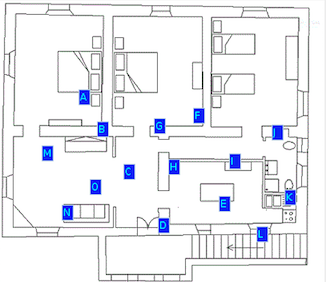
\includegraphics[width=\linewidth, height=8cm]{pictures/puttiArea.png}
\caption{The archaeological site on the map}
\label{fig:puttiArea}
\end{figure}

The sequence diagrams related to this application are the same shown in Section \ref{alfalfa}. 
The only difference is that now the application does not require the repetition of the missions.
This leads the Main Application to end the execution flow when the Mission reaches a successful evaluation.

\subsection{PM10}

The PM10\cite{pm10} application is used to build 3D maps of pollution concentration in the atmosphere. 
Initially, there is a predefined 3D grid over which drones are sent to sample the quantity of pollution.
So the drones build a spatial profile of pollution concentration and compute gradients among the areas of higher concentration.
Finally the drones are sent along this gradients to sample the pollution concentration, in order to improve the spatial profile representation.
Any two consecutive samples must be gathered within a given time bound, otherwise the system will take care of speeding up the execution.




For the measurements of pollution quantity, the \textit{Measure} action can be used.
\\

The spatial grid must be manually built by the user, organizing the Trips of each Mission on the map he's provided with.
\\

The data collected by the drones are not photos anymore, but a \textit{pollutionQuantity} value which indicates the percentage of pollution in that area.
\\

Then, thanks to the Mission Evaluator blocks, the \textit{pollutionQuantity} variables are confronted and the gradients between areas of higher concentration are computed.
So new drones will be sent along this gradients, improving the spatial profile.
\\

As for the Aerial Mapping application, shown in section \ref{aerialMapping}, Pluto cannot fulfill the time constraint between two consecutive pollution samples.
As already explained, the timer of Pluto starts when the drone leaves the base station and ensures that it will perform the action within that time interval, but there is no way to constrain the time between two consecutive samples.
\\


Below there is our implementation of a possible Evaluator algorithm:
\\

\begin{lstlisting}
		String result = null;

		// building a new map with only the trip-measure couples of the mission
		// to evaluate
		Map<Trip, Integer> missionMap = new Map<Trip, Integer>();
		for (Map.Entry<Trip, Object> entry : dataMap.entrySet()) {
			if (missionToEvaluate.getCompletedTrips().contains(entry.getKey())) {
				missionMap.put(entry.getKey(), (Integer) entry.getValue());
			}
		}

		// this method use the Trip location and the pollution measure to
		// calculate
		// the gradients and then return a list of String that indicates
		// the positions of these gradients
		List<String> gradientsPositions = calculateGradients(missionMap);

		for (String position : gradientsPositions) {

			// create a new Trip to calculate pollution at the gradient position
			Trip trip = new Trip();
			trip.setName("GradientTrip");
			trip.setTargetLocation(position);
			trip.setAction(Action.MEASURE);
			trip.setStatus(Trip.WAITING);

			// add this new trip to the list of trips to be executed
			missionToEvaluate.getTrips().add(trip);
			// set the mission status to STANDBY, since there are new trips to perform
			missionToEvaluate.setStatus(Mission.STANDBY);
			
		}
			
		// set the result of the evaluation
		result = "Success";
		return result;
\end{lstlisting}


Now we show the execution of the PM10 application with Pluto in a particular scenario:
we have 5 drones and we want to measure the pollution quantity in the area shown in figure \ref{fig:pm10Area} using all of them.
As usual, the user has to create 5 Missions and has to choose the locations of the area to sample through the map on the Trips Page of each Mission.
In this way, five drones will monitor simultaneously the area to sample.

\begin{figure}[H]
\centering
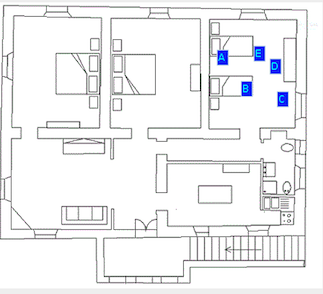
\includegraphics[width=\linewidth, height=8cm]{pictures/pm10Area.png}
\caption{The area to sample on the map}
\label{fig:pm10Area}
\end{figure}

As for the Aerial Mapping\cite{putti} application, the repetition of missions is not required.
So the sequence diagrams don't change and the reader can see them in sections \ref{alfalfa} and \ref{aerialMapping}.


\subsection{PURSUE}\label{PURSUE}


The PURSUE application\cite{pursue} is representative of surveillance applications. A team of drones monitor an area and they have to follow moving objects which pass through, taking a picture of each one of them when they enter in the camera field.
To do so, drones can operate in two distinct modes: when in "patrolling mode" they simply inspect an area, while when an object is found they switch to "pursuing mode" and start to follow the object.
Since an object could move faster than the drones, no drone can follow it constantly, the system must take care of switching between the real drones in order to constantly follow the target.
There are time constraints to respect between the detection of a moving object and when its picture is taken and, in case of violations,every tracked object with at least one acquired picture is released from tracking, to regain the drone resources and lower the acquisition latency for the next object.
\\

The PURSUE application represents a limit for the Pluto programming framework.
Indeed, in our model, the drones perform their action only at the end of the Trip, so it's not possible for them to actively take a picture in the very same moment the moving object enters in the camera field.
This problem can be lowered by inserting a lot of trips in the area to monitor, with strict time constraints on them, in order to obtain a lot of pictures of the monitored area.
But in this way, not only it's not sure to capture the moving object, but there will be a lot of useless empty pictures.
And, above all, there is still no way for the drones to actively follow the moving objects.

We can conclude that the PURSUE application is too "dynamic" for the Pluto programming framework, and this can be an hint for a future expansion of our work.


\newpage

The applications described above were already developed and tested with other systems, like Karma\cite{karma} and Voltron\cite{voltron}, but we also developed new applications and tested our framework on them:
the Object-finder (OF), the Warehouse item-finder (WIF) and the Drugs distribution(DD).
\\

The three applications are modeled by the same Pluto Editor graph, shown in figure \ref{fig:plutoGraph}:

\begin{figure}[H]
  \centering
  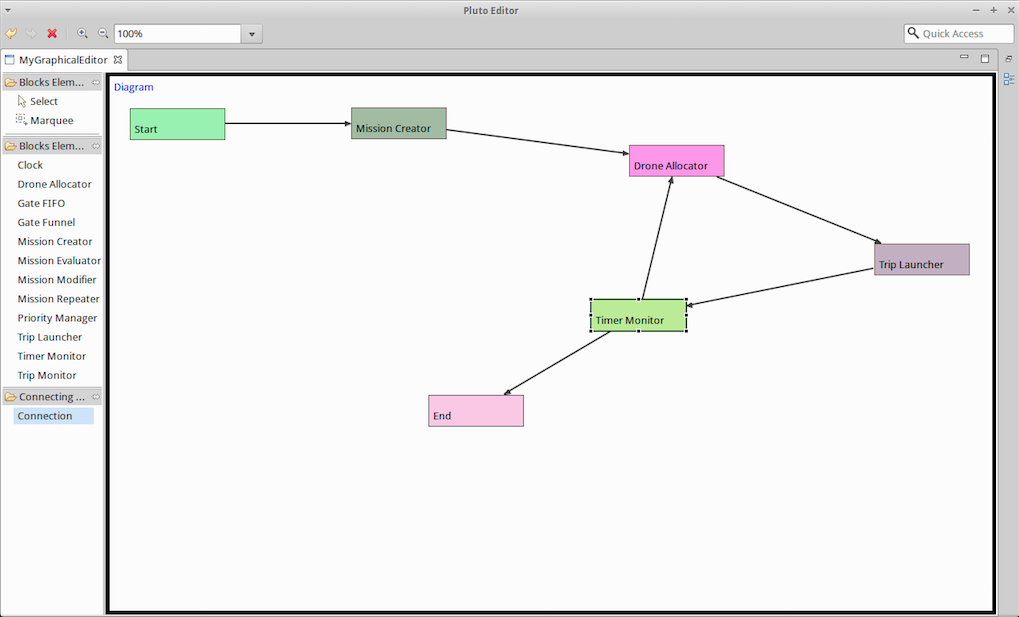
\includegraphics[width=\linewidth]{pictures/EditorScreen.png}
  \caption{The Pluto graph of the OF,WIF and DD applications}
  \label{fig:plutoGraph}
\end{figure}

In the following sections we describe these applications in details, also using a visual representation of their behavior, and a sequence diagram to make understand better the whole functioning of each one of them.

\newpage

\subsection{Object-finder (OF)}

This application help users to find various objects, like shoes, keys, books, in a domestic fashion:

\begin{itemize}
\itemsep2pt
\item{
the user decides which item wants the drones to look for and the area to be inspected
}
\item{
the main system organizes the team of drones, sending them on the specified locations
}
\item{
the drones fly to the assigned location and, if found, bring the objects back to the user
}
\end{itemize}


\begin{figure}[H]
  \centering
  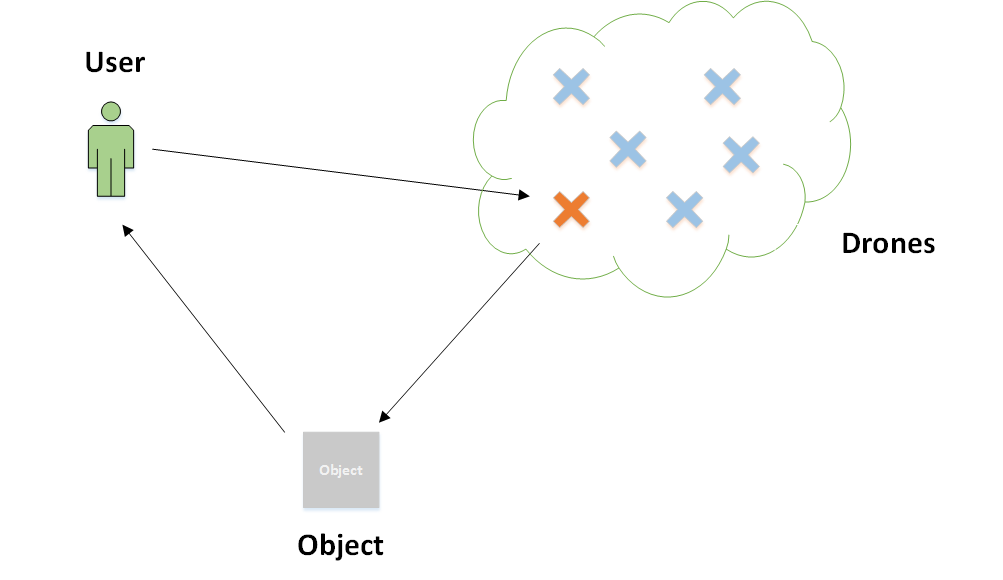
\includegraphics[width=\linewidth]{pictures/OF.png}
  \caption{The basic functioning of the Object-finder application}
  \label{fig:OF}
\end{figure}



\newpage

\subsection{Warehouse item-finder (WIF)}

This application help users to manage a warehouse, bringing a list of objects to the them:

\begin{itemize}
\itemsep2pt
\item{
the user makes a list of needed items and writes it on his laptop, tablet or smartphone}
\item{
the main system organizes the drones and decide which one will take each item in the list
}
\item{
the drones fly to the assigned objects and bring them back to the user
}

\end{itemize}


\begin{figure}[H]
  \centering
  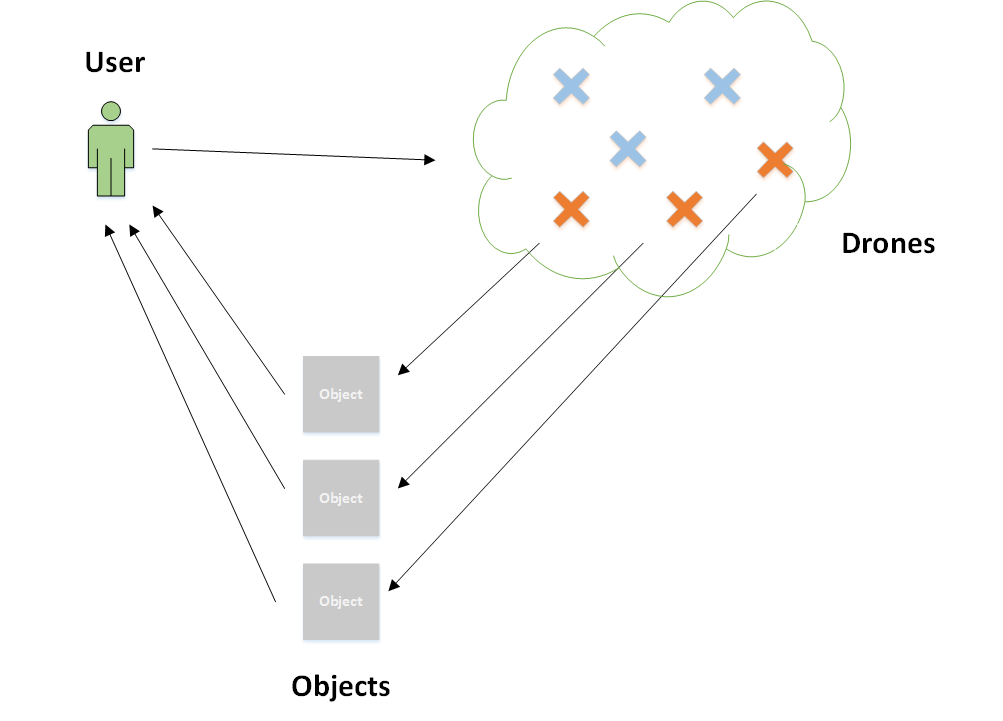
\includegraphics[width=\linewidth]{pictures/WIF.png}
  \caption{The basic functioning of the Warehouse item-finder application}
  \label{fig:WIS}
\end{figure}


\newpage

\subsection{Drugs distribution (DD)}\label{dd}

This application help nurses in assisting elder people to take their daily medicines, in an hospice context:

\begin{itemize}
\itemsep2pt
\item{
the nurses prepare some little boxes with each patient’s daily medicine
}
\item{
each drone, at the right time of the day, brings the box to its assigned patient
}
\item{
after carrying out their action, the drones return to the start location
}

\end{itemize}


\begin{figure}[H]
  \centering
  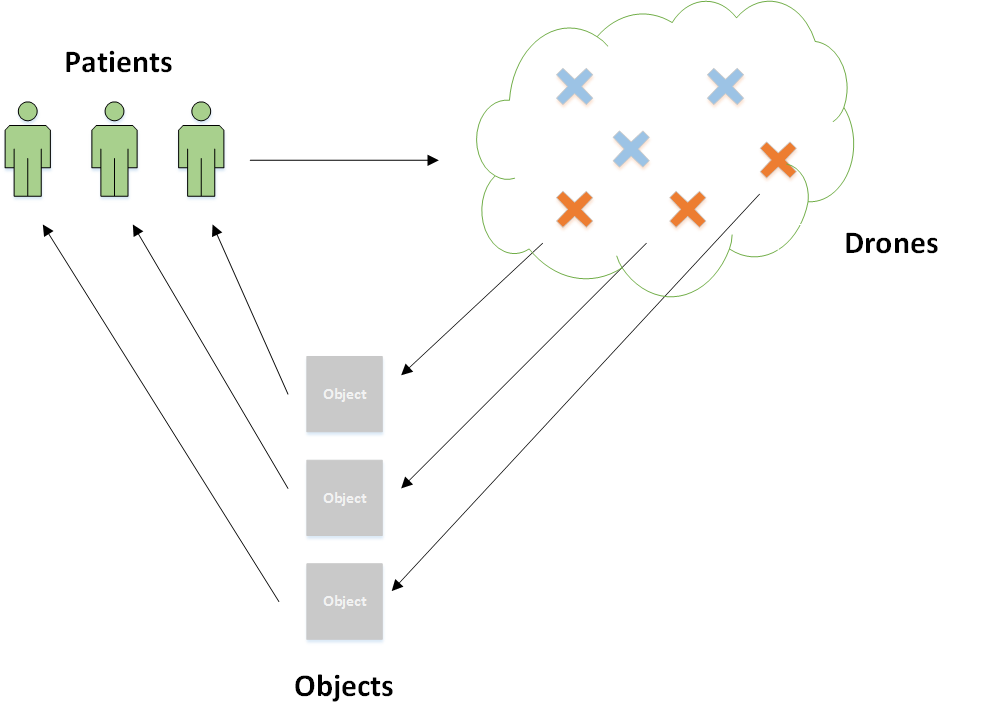
\includegraphics[width=\linewidth]{pictures/DD.png}
  \caption{The basic functioning of the Drugs distribution application}
  \label{fig:DD}
\end{figure}

Here there is a sequence diagram showing the behavior of the three applications:

%sequence

\newpage

\section{Usability of the model}
\label{usability}

To evaluate the concrete usability of the Pluto programming framework, we decided to test it on real people, proposing them two "exercises".
We involved five testers, recruited both in the "Politecnico di Milano" and "SICS Swedish ICT" environment, in order to guarantee a solid development background and to avoid possible lack of programming knowledge.
We created one exercise for each component of Pluto framework.
The first one consists in the development of an application using the Pluto Graphical Editor.
The exercise is split in three levels, starting from a very basic version and going through more difficult versions. Each version asks the user to add a new functionality by using the available components in the Editor.
The second exercise, instead, asks the user to use the generated code from the previous exercise to run the Pluto Main Application, then asks to create some missions and, in the end, to run them.
The application we choose for the exercises is the Drugs Distribution, already described in section \ref{dd}, because it's very suitable for the type of evaluation we want to perform.
Indeed its basic version can be extended with many features, for example using the Mission Modifier block (Section \ref{missionModifier}), and this is exactly our purpose.
The results are shown in section \ref{surveyResult}.
After the execution of the exercises, we asked the users to leave a feedback, proposing them a survey, built according to some metrics that we have defined and that we describe in section \ref{survey}.

\subsection{Proposed exercises}
\label{exercise}

We give the user a complete and sound explanation of the Pluto programming framework, showing how the graphical editor works (shown in Section \ref{plutoGraphicalEditor}) and giving him the list of the available entities (shown in Section \ref{programmingModel}) and of the implemented blocks (shown in Section \ref{functionalBlocks}), together with an explanation of the meaning and functionality of each one.
The same explanations are given for all the components of the Pluto User Application (shown in Section \ref{plutoMainApp}).

\subsubsection{First Exercise}

The exercise proposes the development of the Drugs Distribution application (shown in section \ref{dd}) in three different versions, increasingly harder to implement:

\begin{itemize}
\itemsep2pt
\item{
\textit{basic version}: we ask the user to implement the basic version of the Drugs Distribution application
}
\item{
\textit{medium version}: we ask the user to raise the priority of the failed trips and to re-insert them in the queue of next trips to be launched, and to add a delay for the trips.
}
\item{
\textit{hard version}: we ask the user to add a time constraint within each trip must be completed, that is the same feature implemented by the Timer Monitor block, but using the Mission Modifier block.
}
\end{itemize}

To solve the first part of the exercise, the user has to create the graph shown in figure \ref{fig:firstStep}, that represents the very basic scheme of each application, since it uses only the basic blocks.
Once created the graph, the user has to right click on the panel and choose "generate code" to accomplish the first step of the exercise.
This is a very easy task to perform, but we think it's useful, because make the user confident with the basic features of Pluto, such as the basic blocks and the code generation mechanism.


\begin{figure}[htb]
  \centering
  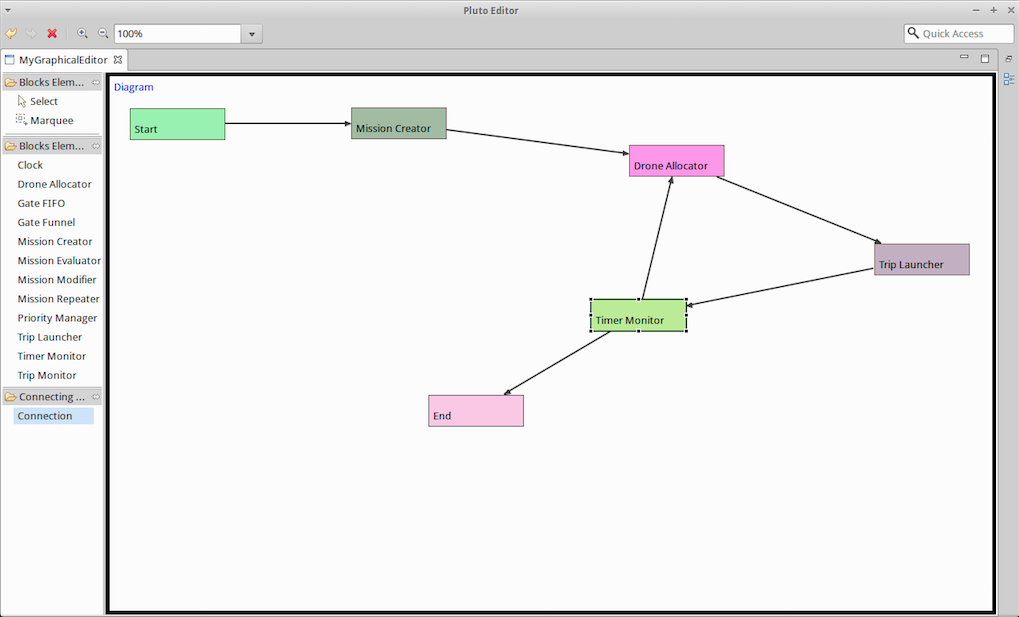
\includegraphics[width=\linewidth]{pictures/EditorScreen.png}
  \caption{Solution of the first step}
  \label{fig:firstStep}
\end{figure}

\newpage

To solve the first part of the second step of the exercise, the user has only to understand that the functionality to add is already implemented by the Priority Manager block, so he has only to add this block to the graph in the right point.
Since we ask him to re-insert the failed trips in the queue of unexecuted trips he has to put the block between the Trip Monitor and the Drone Allocator, as shown in figure \ref{fig:secondStepPriority}.

\begin{figure}[htb]
  \centering
  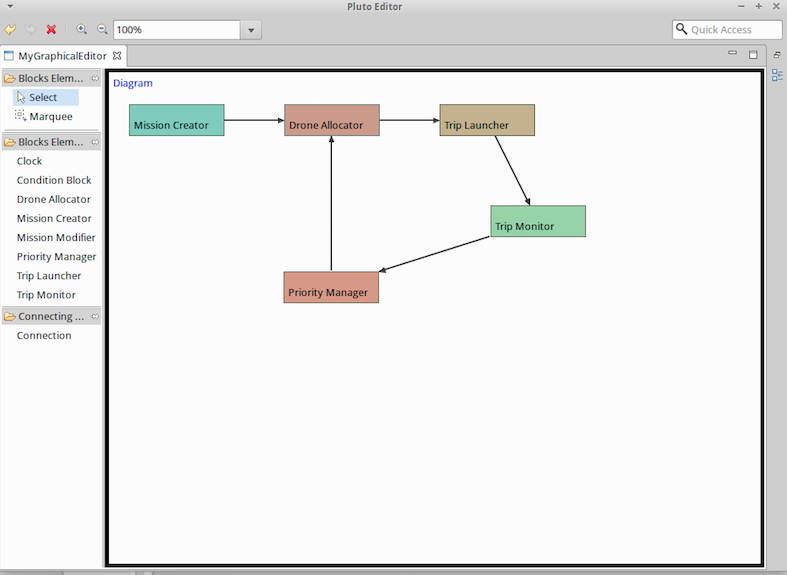
\includegraphics[width=\linewidth,height=7cm]{pictures/secondStep.png}
  \caption{Solution of the second step with Priority Manager}
  \label{fig:secondStepPriority}
\end{figure}

Then to add the Delay feature in the diagram the user needs to do the same thing with the Clock block, that provides the feature to wait for an amount of time, set in the delay attribute of a Trip. This block is taking as input the mission provided by the Trip Monitor and the by the Mission Creator then, after the delay time has passed, gives the mission to the DroneAllocator block, as shown in figure \ref{fig:secondStepClock}.

This is a useful step to compute, because the user learns how to use the connection element, that is a very important feature in the Pluto framework, and also the Priority Manager and Clock blocks.

\begin{figure}[htb]
  \centering
  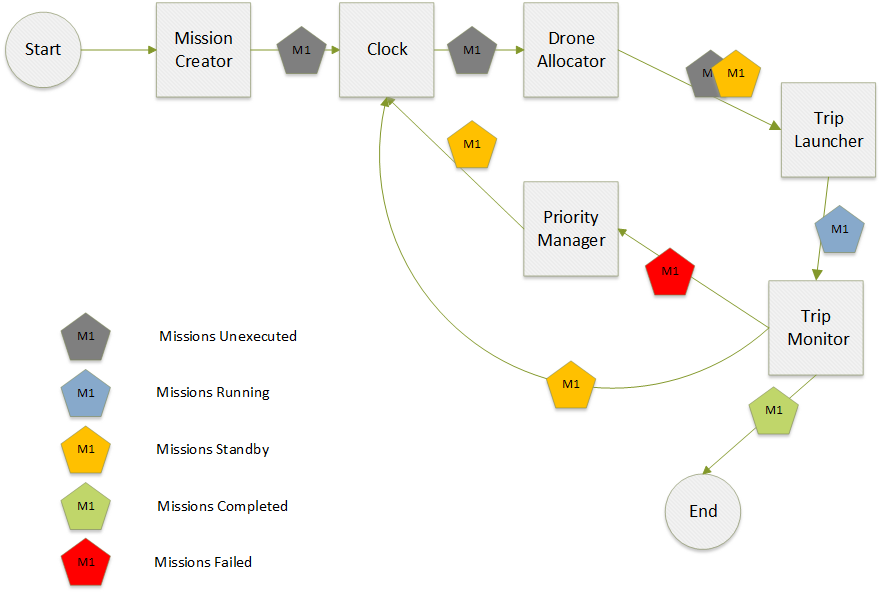
\includegraphics[width=\linewidth,height=7cm]{pictures/secondStepClock.png}
  \caption{Solution of the second step with Clock block}
  \label{fig:secondStepClock}
\end{figure}

\newpage

For the third step, the user has to implement the feature of the Timer Monitor block without using it.
So, he has to use the Mission Modifier block, through which he can insert his code in the application, and put it between the Trip Launcher and GateFIFO blocks, in parallel with the TripMonitor, as shown in figure \ref{fig:thirdStep}.
This is a very useful step to compute, because the user learns how to use Mission Modifier block, which is an important feature of the Pluto Editor, because it allows the programmer to insert his custom code to characterize the application.

\begin{figure}[H]
  \centering
  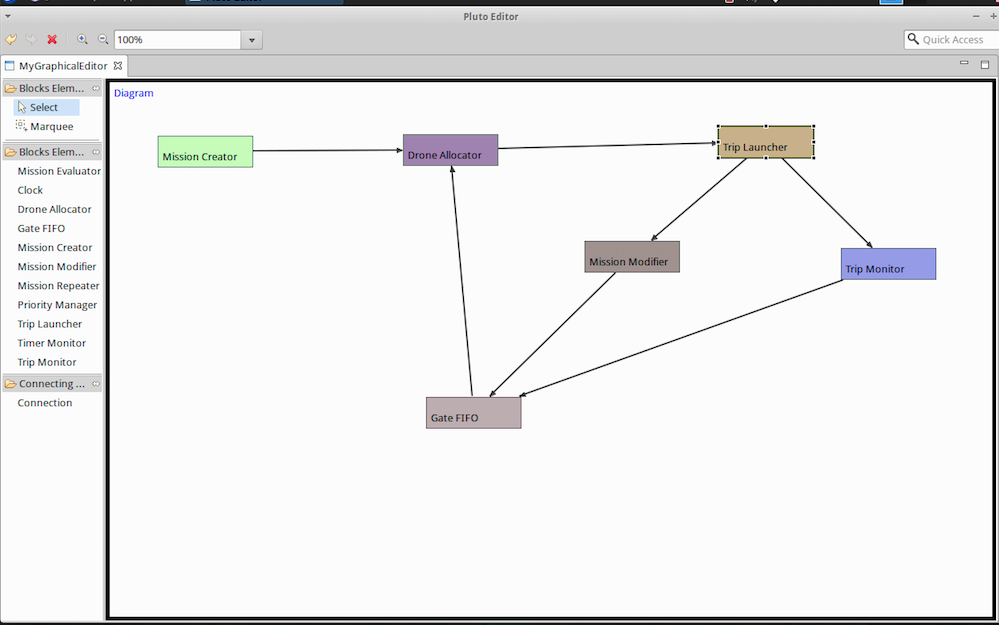
\includegraphics[width=\linewidth, height=8cm]{pictures/thirdStep.png}
  \caption{Solution of the third step}
  \label{fig:thirdStep}
\end{figure}

\subsubsection{Second Exercise}

The main purpose of this exercise is to underline possible issues in the code generated with the Pluto Graphical Editor. We must be sure that all the functionality described by the diagram are enabled in the generated code and that the missions execution will run smooth as the user expects. Any lack in the user experience may compromise the usability of the entire application, so it is important to evaluate the User Interface too. In this way, we check if the visual disposition of the graphics elements is appropriate.
The first step asks every user to create and run the same kind of missions, as described in the following list:

\begin{itemize}
\item Mission 1
	\subitem Trip A -> Action: Take Photo
    \subitem Trip B -> Action: Take Photo
    \subitem Trip C -> Action: Take Photo
\item Mission 2
	\subitem Trip A -> Action: Measure
    \subitem Trip B -> Action: Measure
\item Mission 3
	\subitem Trip A -> Action: Pick Item
    \subitem Trip B -> Action: Release Item
    \subitem Trip C -> Action: Take Photo
    \subitem Trip D -> Action: Measure
\end{itemize}

The location in the map of the Trips was not important while testing, so the tester could decide any place.
In the second step the users were asked to open the Monitor Page and to start the missions following their execution using the provided table and console.
The third step of the exercise consists in calling back the Drone with an RTL command.


\subsection{Evaluation metrics}\label{metrics}

To concretely evaluate the usability of the Pluto programming framework we defined the following metrics, which we applied for both exercises:

\begin{enumerate}
\item {Number of people who correctly solved the first part of the exercise}
\item {Number of people who correctly solved the first and second parts of the exercise}
\item {Number of people who correctly solved the whole exercise}
\item {Mean time for the resolution of the first part of the exercise}
\item {Mean time for the resolution of the second part of the exercise}
\item {Mean time for the resolution of the third part of the exercise}
\item {Mean time for the resolution of the whole exercise}
\item {Number of people who solved the whole exercise, but in a wrong way}
\item {Number of people who could not solve the exercise at all}
\end{enumerate}

Through metrics 1,2 and 3 we can understand which parts of the exercises are not clear for the user and/or too difficult to implement. 
Through metrics 4,5,6 and 7 we can understand, once the user has understood how to implement each feature, how much is difficult to solve each part of the exercises by measuring the time required to solve each step.
Through metrics 8 and 9, finally, we can understand how easy is to confuse the specifications and how many people couldn't solve any step of the exercises.


\subsection{Baseline}

We want to demonstrate the effective usefulness of the Pluto programming framework, so we decide to compare its features with the API of the Crazyflie Nano-quadcopter, which was described in section \ref{crazyflie}.

Actually, the crazyflie is the drone we chose to use for our applications case study, and we want to demonstrate that, without Pluto and using only the Crazyflie API would be more difficult to build the same kind of applications.

So we decide to propose another exercise to our users, but this time they can use only the Crazyflie API and they have a limited amount of time.

The Crazyflie API is written in Python, so we address to people who knows Python language features.

The exercise consists in make the drone moving from a point A to a point B on a map, performing a single Trip.

It may seem easy, but it can can take a long time to fully understand and apply the API in the correct way.


\subsection{User Survey}\label{survey}

Since we want to evaluate the usability of Pluto, we propose a survey to the users, in order to understand how easy it is to use and which modifications should be applied to improve the user experience.

We ask users to tell us how easy was the development of the various steps of the exercises, and to provide us with a feedback on the usability of the editor and the main application underlining any problems found.
We also ask for suggestions to improve the usability of Pluto.

The survey can be found following this link:

\url{https://docs.google.com/forms/d/1b_52e7VLuns6AH1jiT3TeIRZ_KPRTLJYJe9ckrJanWY/viewform?usp=send_form}
\\

Actually, this survey gives us very useful information about the Pluto framework. We can understand how "usable" it is and which modifications should be performed to improve the user's experience, also thanks to the visualization of the answers in a graphical way, shown in the next section, the \ref{surveyResult}.
Through the questions on the exercises development we can understand how difficult it is to create, modify,customize and execute a particular application, validating "on field" the use of the various blocks, especially the Mission Modifier, and the usability of the user interface.

\subsection{Results}\label{surveyResult}

Thanks to the combination of the answers to the user survey of section \ref{survey} and the numeric data collected according to the metrics defined in section \ref{metrics}, in this section we show the results of the Pluto evaluation.
We make use of graphical representation in order to make the results clearer and easily understandable by everyone.
The metrics data are put into the table \ref{surveyTable}, while the results of the user survey are presented with graphics.
\\

\begin{table} [htdp]
\centering
\caption{The values of the metrics for the two exercises}
\label{surveyTable}
    \begin{tabular}{|l|c|c|c|c|c|c|c|c|c|}
    \hline
    Metric & 1 & 2 & 3 &  4 &  5 & 6 &  7 & 8 & 9\\ \hline
    Exercise 1 & 5 & 5 & 5 & 10 mins & 10 mins & 20 mins & 40 mins & 0 & 0 \\ \hline
    Exercise 2 & 5 & 5 & 5 & 5 mins & 5 mins & 5 mins & 15 mins & 0 & 0
     \\ \hline
     \end{tabular}
    \end{table}


A graphical representation of the answers to the user survey can be found at the following link:
\\

\url{https://docs.google.com/forms/d/1b_52e7VLuns6AH1jiT3TeIRZ_KPRTLJYJe9ckrJanWY/viewanalytics}
\newpage

Examining both the user survey and the results of the evaluation metrics, we can say that Pluto is quite easy to use.
Indeed, all the five testers managed to solve the two exercises, and, through the survey, they stated that Pluto is easily usable and its functioning is quite fast to understand.
They also give some suggestions, especially on the Pluto Main Application, which made us improve some features that appeared tricky or not easily understandable.


\newpage

\section{Performance evaluation}\label{performance}

In order to strengthen the evaluation of Pluto, after the user study, described in Section \ref{usability}, we evaluated some quantitative metrics. These metrics are divided in two main types: software metrics and resources consumption metrics. The former let us know the complexity of our software.
On the other hand, the latter are useful to underline possible issues at run-time, such as thread deadlock or a too high memory consumption.
\\

Since our framework is composed by two main components (the Graphical Editor and the Main Application) we decided to split this evaluation in two parts: this means that each kind of evaluation was performed on the Pluto Graphical Editor first and then on the Pluto Main Application.
To help us in this procedure we used a very useful tool called VisualVM, shown in figure \ref{fig:visualVM}. 

\begin{figure}[H]
  \centering
  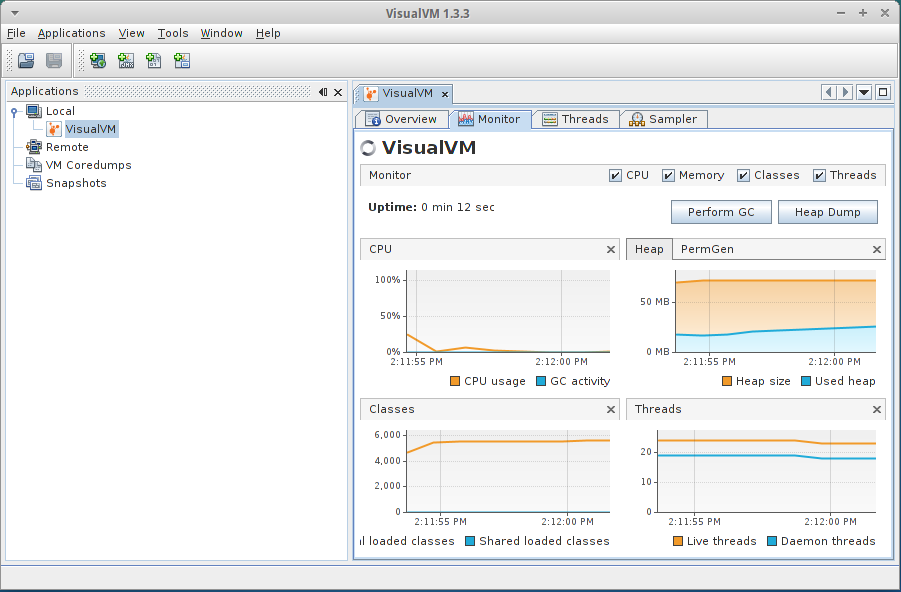
\includegraphics[width=\linewidth]{pictures/visualVM.png}
  \caption{VisualVM interface}
  \label{fig:visualVM}
\end{figure}

It let the user have a global monitoring of the running Java application in your local Java Virtual Machine, at run-time. Furthermore, it has a useful feature that records the profiling of an application in a dump file so that the user can compare different dump files concerning different application sessions.
Finally, in the Result section \ref{metricsResult}, we describe the outcome of the tests for the Pluto Graphical Editor and the Pluto Main Application separately.

\subsection{Software Metrics}

The software metrics let us understand the complexity of the software.
We decided to record this information for each component of the Pluto Framework, because it lets us to understand how much expandable it is and then how much effort a different developer should spend to add new features in the future.
\\

These parameters are:

\begin{itemize}
\item Total Lines Of Code (LOC)
\item Number of attributes
\item Average methods per class
\item Number of classes
\item Number of methods
\end{itemize}

\subsection{Resources Consumption}

The resources consumption metrics are those parameters measured at run-time, during the execution of the software.
With this evaluation we checked if the Pluto framework generates any performance issues, because of a too high requirement of resources. 
\\
Furthermore, due to the team level approach we have chosen, as said in Chapter \ref{cap3}, it is important to verify if critical issues happen during the normal execution because the central brain introduce a single point of failure. It is essential to avoid any bottleneck situations.
These metrics are:

\begin{itemize}
\item CPU Load
\item Memory Consumption
\item Live Threads
\end{itemize}

The profiling of the application was done on a machine with these specifications:

\begin{itemize}
\item CPU: Intel i7 2640
\item RAM: 4GB
\item VGA: Nvidia GeForce 610M
\item SSD: Kingston 120GB
\item OS: Xubuntu 14.04
\item Java: JDK 1.7
\end{itemize}

Concerning the Pluto Graphical Editor, we measured these parameters while generating the source code of the Main Application from an increasingly more complex drawing. 
We raised step by step two parameters: the number of blocks and the number of connections.
At first we fixed the former and we incremented the latter by a step of 5, starting from 1 connection. Then we did the same operation fixing the number of connections and raising the number of blocks by 5, now starting from 2 blocks.

\begin{figure}[H]
  \centering
  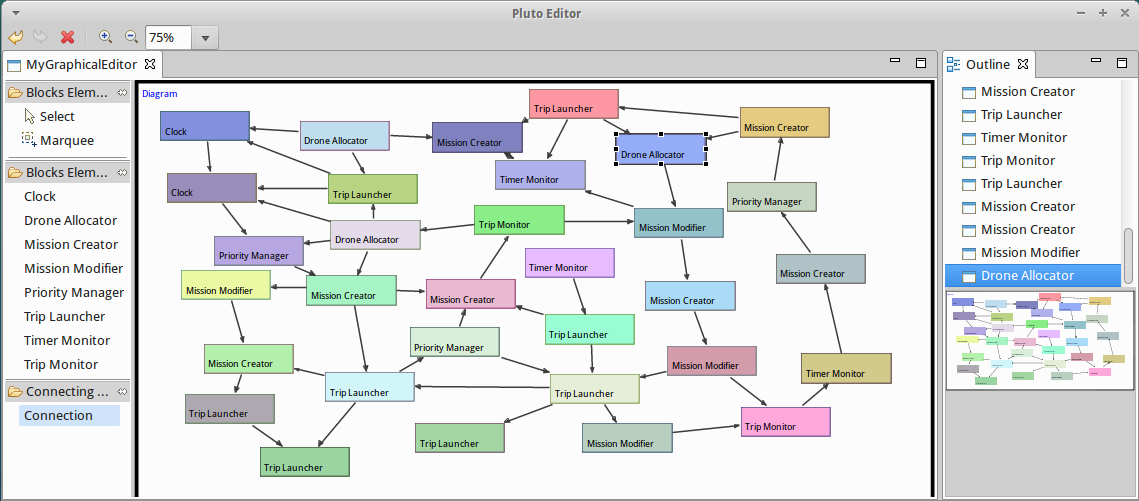
\includegraphics[width=\linewidth]{pictures/stressDiagram.png}
  \caption{Very Complex Diagram Example}
  \label{fig:stressDiagram}
\end{figure}

Furthermore, we evaluated the same metrics concerning the Main Application.
We decided to focus this evaluation varying 3 important parameters: the number of Mission, the number of Trips related to a single Mission and the number of available Drones. 
We started fixing the number of missions and trips varying instead the number of drones. Then we fixed the missions and the drones varying the trips. In the end we fixed the trips and the drones varying the number of missions.
In this way, we could evaluate the performance of the Main Application in an accurate way.
The results are shown in next section \ref{metricsResult}.

\subsection{Results}
\label{metricsResult}

In this section we show the results of the software and resources consumption evaluation. First of all, we evaluated the software complexity of the Pluto framework, according to some important software metrics. The table \ref{table:metricsTable} proposes the results.

\begin{table}[htdp]
\centering
\begin{tabular}{|l|c|c|}
\hline
& Main Application & Graphical Editor \\
\hline
Total lines of code & 2132 & 5072 \\
\hline
Number of classes & 48 & 129 \\
\hline
Number of attributes & 104 & 141 \\
\hline
Number of methods & 197 & 569 \\
\hline
Weighted methods per class & 325 & 848 \\
\hline
\end{tabular}
\caption{The metrics concerning the two Pluto components}
\label{table:metricsTable}
\end{table}

Thanks to these measures, we can make some considerations about the size and the spent effort of the Pluto framework.
\\
Concerning the Main Application, these values are dependent from the diagram generation process because the amount of the generated surplus code doesn't exceed the 2-3\% of the total lines of code of the template Main Application. Indeed the generation adds no more than 50 lines.
\\
Instead, the Graphical Editor has a higher volume than the Main Application, with all the measured values doubled. 
This can be explained by the fact that, to develop the Editor, we based our code on Eclispe GEF Framework.
Then most of the classes, have inherited from other parent classes inside this framework and we inherited its complexity too.
\\
The higher size explains also the time we spent to develop the Graphical Editor and the time needed to add new features during the software revision steps. Indeed we found the GEF framework a bit hard to maintain.
\\
% SPIEGARE PERCHè LE LINEE DI CODICE SONO NORMALI

In the end, we present the results concerning the resources consumption of the two Pluto framework components.
\\
Starting from the Graphical Editor, the diagrams in picture \ref{fig:editorHWMetrics} describe the resources consumption when the connections number raise with fixed number of blocks and when increasing the blocks amount with fixed connections.

\begin{figure}
\centering
\begin{subfigure}[b]{0.3\textwidth}
\centering
  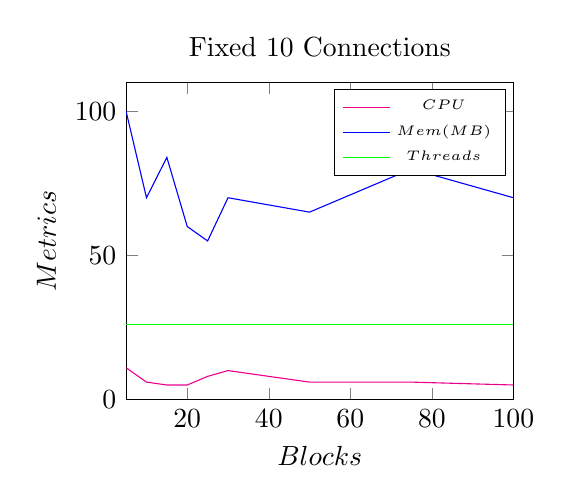
\begin{tikzpicture}
    \begin{axis}[xmin=5,xmax=100,
    ymin=0,ymax=110,
    xlabel=$Blocks$,ylabel=$Metrics$,
    title={Fixed 10 Connections},width=6.5cm,
    legend style={font=\tiny}]
    \addplot [color=magenta]
    coordinates
    {(5, 11) (10, 6)
    (15, 5) (20, 5)
    (25, 8) (30, 10)
    (50, 6) (75, 6) (100, 5)};
    \addplot [color=blue]
    coordinates
    {(5, 100) (10, 70)
    (15, 84) (20, 60)
    (25, 55) (30, 70)
    (50, 65) (75, 80) (100, 70)};
    \addplot [color=green]
    coordinates
    {(5, 26) (10, 26)
    (15, 26) (20, 26)
    (25, 26) (30, 26)
    (50, 26) (75, 26) (100, 26)};
    \legend{$CPU$,$Mem (MB)$,$Threads$}
    \end{axis}
  \end{tikzpicture}
\end{subfigure}\hfill
\begin{subfigure}[b]{0.3\textwidth}
\centering
  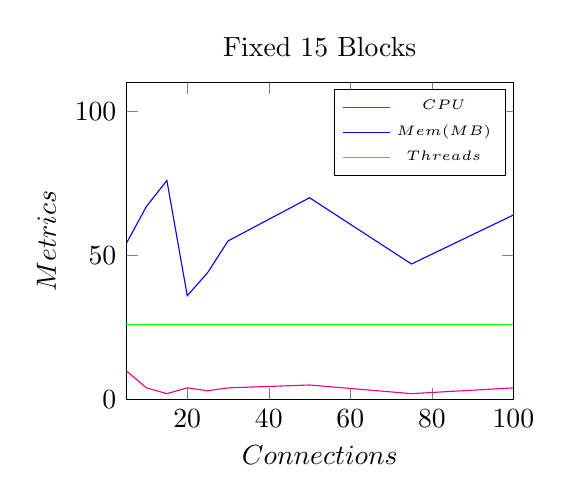
\begin{tikzpicture}
    \begin{axis}[xmin=5,xmax=100,
    ymin=0,ymax=110,
    xlabel=$Connections$,ylabel=$Metrics$,
    title={Fixed 15 Blocks},width=6.5cm, legend style={font=\tiny}]
    \addplot [color=magenta]
    coordinates
    {(5, 10) (10, 4)
    (15, 2) (20, 4)
    (25, 3) (30, 4)
    (50, 5) (75, 2) (100, 4)};
    \addplot [color=blue]
    coordinates
    {(5, 54) (10, 67)
    (15, 76) (20, 36)
    (25, 44) (30, 55)
    (50, 70) (75, 47) (100, 64)};
    \addplot [color=green]
    coordinates
    {(5, 26) (10, 26)
    (15, 26) (20, 26)
    (25, 26) (30, 26)
    (50, 26) (75, 26) (100, 26)};
    \legend{$CPU$,$Mem (MB)$,$Threads$}
    \end{axis}
  \end{tikzpicture}
\end{subfigure}\hfill\null
\caption{Resources consumption metrics of Graphical Editor}
\label{fig:editorHWMetrics}
\end{figure}

\newpage

As you can see the Graphical Editor doesn't require a big amount of hardware resources while generating the code, even with complex diagrams.
\\

The Main Application evaluation gave us different results, shown in the following figures.
\\

\begin{figure}[h!]
\centering
  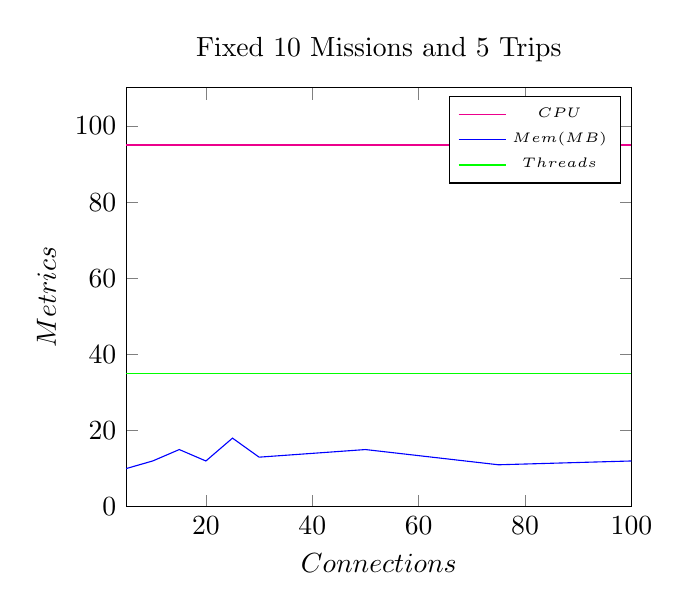
\begin{tikzpicture}
    \begin{axis}[xmin=5,xmax=100,
    ymin=0,ymax=110,
    xlabel=$Connections$,ylabel=$Metrics$,
    title={Fixed 10 Missions and 5 Trips},width=8cm, legend style={font=\tiny}]
    \addplot [color=magenta]
    coordinates
    {(5, 95) (10, 95)
    (15, 95) (20, 95)
    (25, 95) (30, 95)
    (50, 95) (75, 95) (100, 95)};
    \addplot [color=blue]
    coordinates
    {(5, 10) (10, 12)
    (15, 15) (20, 12)
    (25, 18) (30, 13)
    (50, 15) (75, 11) (100, 12)};
    \addplot [color=green]
    coordinates
    {(5, 35) (10, 35)
    (15, 35) (20, 35)
    (25, 35) (30, 35)
    (50, 35) (75, 35) (100, 35)};
    \legend{$CPU$,$Mem (MB)$,$Threads$}
    \end{axis}
  \end{tikzpicture}
  \caption{Evaluation results of Main Application with fixed missions and trips}
  \label{fig:mainApp1}
\end{figure}

The diagram \ref{fig:mainApp1} describes the resources consumption of the Main Application with a fixed number of missions and trips and a raising number of drones. We created 10 missions with 5 trips each.
\\

\begin{figure}[h!]
\centering
  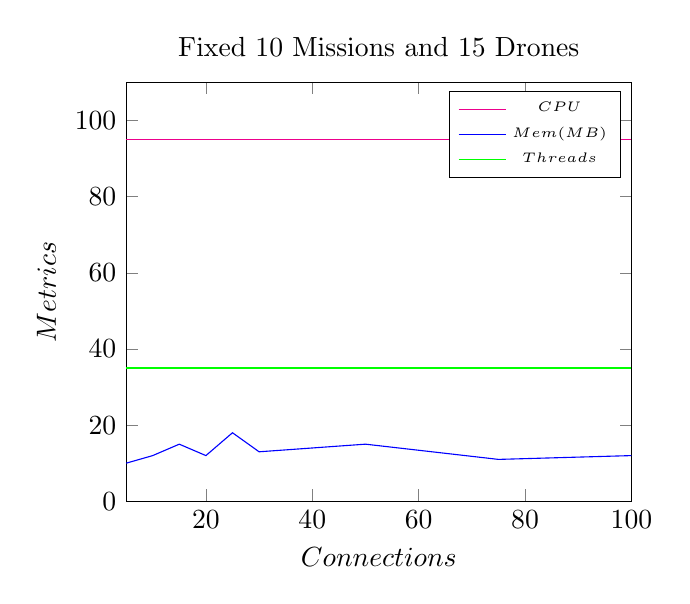
\begin{tikzpicture}
    \begin{axis}[xmin=5,xmax=100,
    ymin=0,ymax=110,
    xlabel=$Connections$,ylabel=$Metrics$,
    title={Fixed 10 Missions and 15 Drones},width=8cm, legend style={font=\tiny}]
    \addplot [color=magenta]
    coordinates
    {(5, 95) (10, 95)
    (15, 95) (20, 95)
    (25, 95) (30, 95)
    (50, 95) (75, 95) (100, 95)};
    \addplot [color=blue]
    coordinates
    {(5, 10) (10, 12)
    (15, 15) (20, 12)
    (25, 18) (30, 13)
    (50, 15) (75, 11) (100, 12)};
    \addplot [color=green]
    coordinates
    {(5, 35) (10, 35)
    (15, 35) (20, 35)
    (25, 35) (30, 35)
    (50, 35) (75, 35) (100, 35)};
    \legend{$CPU$,$Mem (MB)$,$Threads$}
    \end{axis}
  \end{tikzpicture}
  \caption{Evaluation results of Main Application with fixed missions and drones}
  \label{fig:mainApp2}
\end{figure}

The diagram \ref{fig:mainApp2} describes the resources consumption of the Main Application with a fixed number of missions and drones and a raising number of trips for each mission. We created 10 missions and made available 15 drones.
\newpage

\begin{figure}[h!]
\centering
  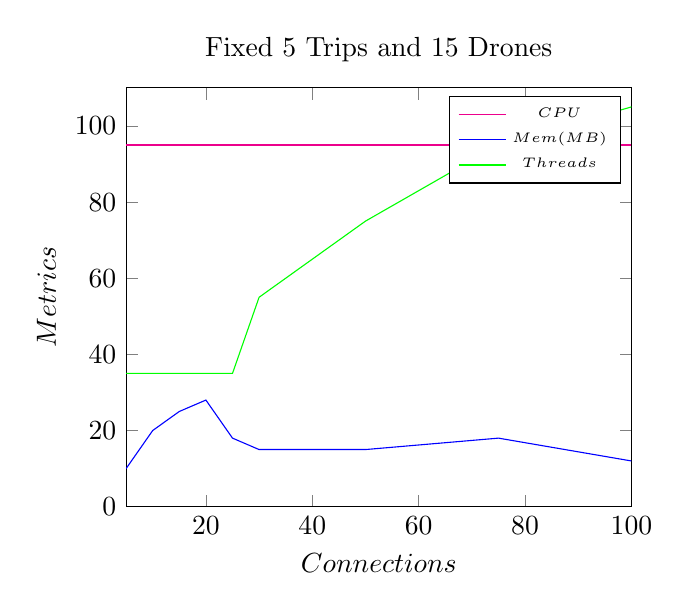
\begin{tikzpicture}
    \begin{axis}[xmin=5,xmax=100,
    ymin=0,ymax=110,
    xlabel=$Connections$,ylabel=$Metrics$,
    title={Fixed 5 Trips and 15 Drones},width=8cm, legend style={font=\tiny}]
    \addplot [color=magenta]
    coordinates
    {(5, 95) (10, 95)
    (15, 95) (20, 95)
    (25, 95) (30, 95)
    (50, 95) (75, 95) (100, 95)};
    \addplot [color=blue]
    coordinates
    {(5, 10) (10, 20)
    (15, 25) (20, 28)
    (25, 18) (30, 15)
    (50, 15) (75, 18) (100, 12)};
    \addplot [color=green]
    coordinates
    {(5, 35) (10, 35)
    (15, 35) (20, 35)
    (25, 35) (30, 55)
    (50, 75) (75, 95) (100, 105)};
    \legend{$CPU$,$Mem (MB)$,$Threads$}
    \end{axis}
  \end{tikzpicture}
  \caption{Evaluation results of Main Application with fixed trips and drones}
  \label{fig:mainApp3}
\end{figure}

The diagram \ref{fig:mainApp3} describes the resources consumption of the Main Application with a fixed number of trips and drones and a raising number of missions. We created 5 trips for each mission and made available 15 drones.
\\

As you can see, the general consumption is almost the same for each situation: there is a low request of memory, a limited number of live threads, and a quite high consumption of the CPU.
\\

It's important to put in evidence an unexpected situation regarding the third experiment, the one in which we fixed the number of trips and drones.
When we reached a certain number of missions, the system fell in a deadlock situation.
For example, whit 15 drones and 5 trips, we had no problems until we reached 25 missions.
Then, when we raised the amount of available drones, for example setting it to 20, the system didn't fall in the deadlock situation and all the missions were completed successfully.
\\
This problem put in evidence a possible dependency between the number of missions created and the number of available drones.
The causes of this issue could be hardware related, meaning that a more powerful machine could be able to complete all the missions even with a low number of available drones.